\documentclass[UTF8]{ctexbook}

\usepackage[]{ctex}
\usepackage{amsmath}
\usepackage{geometry}
\usepackage[colorlinks=true]{hyperref}
\usepackage{indentfirst}
\usepackage[center]{titlesec}
\usepackage{graphicx}
\usepackage{esint}
\usepackage{cases}

\geometry{left=1cm,right=1cm,top=3cm,bottom=3cm}
\title{db的日常笔记}
\date{最后的编译日期:\today}
\author{dbydd}    
\kaishu
\setlength{\parindent}{2em}
\titleformat{\section}[block]{\LARGE\itshape\mdseries}{\arabic{section}}{1em}{}[]
\titleformat{\subsection}[block]{\Large\itshape\mdseries}{\arabic{section}.\arabic{subsection}}{1em}{}[]
\titleformat{\subsubsection}[block]{\large\itshape\mdseries}{\arabic{section}.\arabic{subsection}.\arabic{subsubsection}}{1em}{}[]
\titleformat{\paragraph}[block]{\small\bfseries}{[\arabic{paragraph}]}{1em}{}[]
\setcounter{secnumdepth}{3}
\setcounter{tocdepth}{3}

\newcommand{\limNormal}[1]{\lim\limits_{#1}}
\newcommand{\myLimToZero}{\limNormal{x \to 0}}
\newcommand{\myLimToInf}{\limNormal{x \to \infty}}
\newcommand{\derivative}{^\prime}
\newcommand{\myLeftRightArrow}{$\Leftrightarrow$}
\newcommand{\myRightArrow}{$\Rightarrow$}
\newcommand{\mathCombination}[2]{C_{#1}^{#2}}
\newcommand{\mathPermutation}[2]{P_{#1}^{#2}}
\newcommand{\UpDownSum}[2]{$\sum_{#1}^{#2}$}
\newcommand{\fDerivative}[1]{\fint\derivative(#1)}
\newcommand{\defFunction}[1]{\fint(#1)}
\newcommand{\definiteIntegral}[2]{\int^{#1}_{#2}}

\begin{document}
\pagestyle{empty}{
  \maketitle
  \paragraph{todos}{
    泰勒公式
  }
  \tableofcontents
  \newpage
}
\setcounter{page}{1}
\chapter{数学}{
\section{基本概念}{
\subsection{六大基本初等函数}{
  常数函数,幂函数,指数函数,对数函数,三角函数
}

\subsection{介值定理}{
在数学分析中,介值定理(英语:intermediate value theorem,又称中间值定理)描述了连续函数在两点之间的连续性:

假设有一连续函数$\fint:[a,b]\rightarrow \mathbf{R}$, 且假设$\fint(a)<\fint(b)$, 若对任意数$u$满足$\fint(a)<u<\fint(b)$,则存在一点$c,a<c<b$,使得$\fint(c) = u$,当$\fint(a)>\fint(b)$时也有类似叙述

直观的比喻:这代表在$[a,b]$区间上可以画出一条连续曲线,而不让笔离开纸面。
\newline

定理:

假设$I = [a,b]$是一个实数里的闭区间,而$f:I\rightarrow\mathbf{R}$是连续函数,那么其像集$\fint(I)$也是区间。他或者包含$[\fint(a),\fint(b)]$(如果$\fint(b)\leq\fint(a)$)。换言之:

$\fint(I)\supseteq[\fint(a),\fint(b)]$。

或:

$\fint(I)\supseteq[\fint(b), \fint(a)]$。

介质定理通常以下述等价的形式表述:假设$f:I\rightarrow\mathbf{R}$是连续函数,且实数$u$满足$\fint(a)<u<\fint(b)$或$\fint(a)>u>\fint(b)$,则存在$c\in(a,b)$使得$\fint(c) = u$

图示:
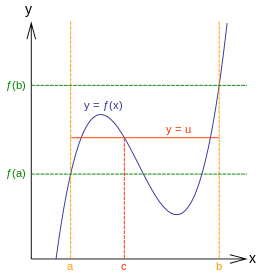
\includegraphics{resources/Intermediatevaluetheorem.png}
}

\subsection{二项式定理}{
  $(x + y)^n = x^n + \mathCombination{n - 1}{n}(x^{n-1} y) + \mathCombination{n - 2}{n}(x^{n-2} y^2) + \dots + y^n$
}

\subsection{排列组合}{
  排列:$\mathPermutation{m}{n} = \frac{m!}{(m-n)!}$

  组合:$\mathCombination{m}{n} = \frac{\mathPermutation{m}{n}}{m!} = \frac{n!}{m!(n-m)!}$
}

\subsection{零散的定义}{
  \begin{enumerate}
    \item 有界:$\exists\epsilon,f(x) < \epsilon\quad(-\infty < x < \infty )$
  \end{enumerate}
}

\subsection{零散的思想}{
  \begin{enumerate}
    \item 正变换是数学的重要工具,三角变换是只变其形不变其质的。三角变换常常先寻找式子所包含的各个角之间的联系,并以此为依据选择可以联系它们的适当公式,通过换元法把三角恒等变换问题转化为代数恒等变换问题。
  \end{enumerate}
}
}

\section{三角函数}{
三角函数一般由单位圆引出,如下:

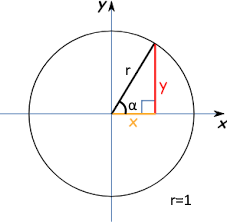
\includegraphics{resources/UnitCircle.png}

\subsection{正三角函数}{
  $\sin{\alpha} = \frac{y}{r}$

  $\cos{\alpha} = \frac{x}{r}$

  $\tan{\alpha} = \frac{y}{x}$
}
\subsection{反三角函数}{
  $\cot{\alpha} = \frac{1}{\tan{\alpha}}$

  $\sec{\alpha} = \frac{1}{\cos{\alpha}}$

  $\csc{\alpha} = \frac{1}{\sin{\alpha}}$
}

\subsection{和差化积}{
  $\sin{\alpha}+\sin{\beta} = 2\sin{\frac{\alpha + \beta}{2}}\cos{\frac{\alpha - \beta}{2}}$

  $\cos{\alpha}+\cos{\beta} = 2\cos{\frac{\alpha + \beta}{2}\cos{\frac{\alpha-\beta}{2}}}$

  $\cos{\alpha}-\cos{\beta} = -2\sin{\frac{\alpha + \beta}{2}}\cos{\frac{\alpha - \beta}{2}}$

  $\sin{\alpha}-\sin{\beta} = 2\sin{\frac{\alpha + \beta}{2}}\cos{\frac{\alpha - \beta}{2}}$

  $\tan\alpha - \tan\beta = \tan(\alpha - \beta) \cdot (1 + \tan\alpha\tan\beta)$
}

\subsection{积化和差}{
  $\cos(\alpha + \beta) = \cos{\alpha}\cos{\beta} - \sin{\alpha}\sin{\beta}$

  $\cos(\alpha - \beta) = \cos{\alpha}\cos{\beta} + \sin{\alpha}\sin{\beta}$

  $\sin(\alpha \pm \beta) = \sin{\alpha}\cos{\beta} \pm \cos{\alpha}\sin{\beta}$

  $\tan(\alpha + \beta) = \frac{\tan\alpha + \tan\beta}{1 - \tan\alpha\tan\beta}$

  $\tan(\alpha - \beta) = \frac{\tan\alpha - \tan\beta}{1 + \tan\alpha\tan\beta}$

  $\sin{\alpha}\cos{\beta} = \frac{1}{2}[\sin{(\alpha + \beta)} + \sin{(\alpha - \beta)}]$

  $\cos{\alpha}\cos{\beta} = \frac{1}{2}[\cos{(\alpha + \beta)} + \cos{(\alpha - \beta)}]$

  $\sin{\alpha}\sin{\beta} = -\frac{1}{2}[\cos{(\alpha + \beta)} - \cos{(\alpha - \beta)}]$
}

\subsection{诱导公式}{
  \indent 奇变偶不变,符号看象限。
  \subsubsection{第一组诱导公式}{
    $\sin{(2k\pi + \alpha)} = \sin{\alpha}$

    $\cos{(2k\pi + \alpha)} = \cos{\alpha}$

    $\tan(2k\pi + \alpha) = \tan\alpha$

    $\cot(2k\pi + \alpha) = \cot\alpha$
  }

  \subsubsection{第二组诱导公式}{
    $\sin(-\alpha) = -\sin\alpha$

    $\cos(-\alpha) = \cos\alpha$

    $\tan(-\alpha) = -\tan\alpha$

    $\cot(-\alpha) = -\cot\alpha$
  }

  \subsubsection{第三组诱导公式}{
    $\sin(\pi + \alpha) = -\sin\alpha$

    $\cos(\pi + \alpha) = -\cos\alpha$

    $\tan(\pi + \alpha) = \tan\alpha$

    $\cot(\pi + \alpha) = \cot\alpha$
  }

  \subsubsection{第四组诱导公式}{
    $\sin(\pi - \alpha) = \sin\alpha$

    $\cos(\pi - \alpha) = -\cos\alpha$

    $\tan(\pi - \alpha) = -\tan\alpha$

    $\cot(\pi - \alpha) = -\cot\alpha$
  }

  \subsubsection{第五组诱导公式}{
    $\sin(\frac{\pi}{2} - \alpha) = \cos\alpha$

    $\cos(\frac{\pi}{2} - \alpha) = \sin\alpha$

    $\tan(\frac{\pi}{2} - \alpha) = \cot\alpha$

    $\cot(\frac{\pi}{2} - \alpha) = \tan\alpha$
  }

  \subsubsection{第六组诱导公式}{
    $\sin(\frac{\pi}{2} + \alpha) = \cos\alpha$

    $\cos(\frac{\pi}{2} + \alpha) = -\sin\alpha$

    $\tan(\frac{\pi}{2} + \alpha) = -\cot\alpha$

    $\cot(\frac{\pi}{2} + \alpha) = -\tan\alpha$
  }

  \subsubsection{杂项}{
    $a\sin\alpha + b\cos\alpha = \sqrt{a^2 + b^2}\sin(\alpha+\beta)$

    $\cos\alpha = 2cos^2\frac{\alpha}{2} - 1 = 1-2\sin^2\frac{\alpha}{2}$
  }

}

\subsection{倍角公式}{

\subsubsection{二倍角公式}{
  二倍角公式:由两角和公式推出

  $\sin2\alpha = 2\sin\alpha\cos\alpha$

  $\cos2\alpha = \cos^2\alpha - \sin^\alpha = 2\cos^2\alpha - 1 = 1 - 2\sin^2\alpha$

  $\tan2\alpha = \frac{2\tan\alpha}{1 - \tan^2\alpha}$
}

\subsubsection{半倍角公式}{
  半倍角公式:将二倍角公式中的角$2\alpha$看作整体$\beta$,经过变形推出:

  $\sin\frac{\alpha}{2} = \pm\sqrt{\frac{1 - \cos\alpha}{2}}$

  $\cos\frac{\alpha}{2} = \pm\sqrt{\frac{1 + \cos\alpha}{2}}$

  $\tan\frac{\alpha}{2} = \pm\sqrt{\frac{1-\cos\alpha}{1+\cos\alpha}} = \frac{\sin\alpha}{1+\cos\alpha} = \frac{1-\cos\alpha}{\sin\alpha}$

  $\cot\frac{\alpha}{2} = \frac{1+\cos\alpha}{\sin\alpha} = \frac{\sin\alpha}{1-\cos\alpha}$

  $\sec\frac{\alpha}{2} = \frac{\pm\sqrt{\frac{\sec\alpha - 1}{2\sec\alpha}}2\sec\alpha}{\sec\alpha + 1} = \frac{\pm\sqrt{\frac{4\sec^3\alpha + \sec^2\alpha}{2\cos\alpha}}}{\sec\alpha + 1}$

  $\csc\frac{\alpha}{2} = \frac{\pm\sqrt{\frac{\sec\alpha - 1}{2\sec\alpha}}2\sec\alpha}{\sec\alpha - 1} = \frac{\pm\sqrt{\frac{3\sec^3\alpha - \sec^2\alpha}{2\sec\alpha}}}{\sec\alpha - 1}$
}

\subsubsection{n倍角公式}{
$\cos{n\theta} = \sum_{i = 0}^{\frac{n}{2}}[(-1)^i\mathCombination{2i + 1}{n}\cos^{n - 2i}\theta\sin^{2i}\theta]$

$\sin{n\theta} = \sum_{i = 0}^{\frac{n}{2}}[(-1)^i\mathCombination{2i + 1}{n}\cos^{n - 2i - 1}\theta\sin^{2i+1}\theta]$
}

\subsubsection{万能替换公式}{
  万能替换公式:尝试将正常的三角函数用半角公式表示时经过变形推出:

  角$\alpha(\alpha \neq 2k\pi + \pi ,k \in \mathbf{z})$的所有三角比都可以用 $\tan\frac{\alpha}{2}$表示.这组公式叫做万能替换公式

  $\sin\alpha = \frac{2\tan\frac{\alpha}{2}}{1+\tan^2\frac{\alpha}{2}}$

  $\cos\alpha = \frac{1 - \tan^2\frac{\alpha}{2}}{1 + \tan^2\frac{\alpha}{2}}$

  $\tan\alpha \frac{2\tan\frac{\alpha}{2}}{1 - \tan^2\frac{\alpha}{2}}$
}
}

\subsection{三角恒等式}{

  倒数关系:

  $\sin\alpha \cdot \csc\alpha = 1$

  $\cos\alpha \cdot \sec\alpha = 1$

  $\tan\alpha \cdot \cot\alpha = 1$

  商数关系:

  $\tan{x} = \frac{\sin{x}}{\cos{x}}$

  $\cot\alpha = \frac{\cos x}{\sin x}$

  平方关系:

  $\sin^2\alpha + \cos^2\alpha = 1$

  $1 + \tan^2\alpha = \sec^2\alpha$

  $1 + \cot^2\alpha = \csc^2\alpha$

}

\subsection{解斜三角形}{
设三角形$\triangle ABC$,角A、B、C的对边为abc,以A为原点$O$建系,总有以下公式:

$\mathbf{S}\triangle_{ABC} = \frac{1}{2}AB \cdot CD = \frac{1}{2}cb\sin A$,即$\mathbf{S}\triangle_{ABC} = \frac{1}{2}bc\sin A$

同理得:$\mathbf{S}\triangle_{ABC} = \frac{1}{2}\sin B, \mathbf{S}\triangle_{ABC} = \frac{1}{2}ab\sin C$.

这就是说,三角形的面积等于任意两边与他们夹角正弦值的一半。

\subsubsection{正弦定理}
将$\frac{1}{2}bc\sin A = \frac{1}{2}ac\sin B = \frac{1}{2}ab\sin C$三个公式同除$\frac{1}{2}abc$,得:

$\frac{\sin A}{a} = \frac{\sin B}{b} = \frac{\sin C}{c}$, 也可表示为:$\frac{1}{\sin A} = \frac{b}{\sin B} = \frac{c}{\sin C}$

此式表明:在三角形中,各{\bfseries边}与它所对{\bfseries角的正弦}的比相等
}

\subsubsection{余弦定理}{
  由两点间距离公式,得$a = |BC| = \sqrt{(b\cos A - c)^2 + (b\sin A - 0)^2}$

  两边平方并化简得:

  $a^2 = b^2 - 2b\cos A + c^2$

  $b^2 = a^2 + c^2 - 2ac\cos B$

  $c^2 = a^2 + b^2 - 2ab\cos C$

  也可变形化为:

  $\cos A = \frac{b^2 + c^2 - a^2}{2bc}$

  $\cos B = \frac{a^2 + c^2 - b^2}{2ac}$

  $\cos C = \frac{b^2 + a^2 - c^2}{2ab}$
}
\\

\indent这些关系在直角三角形中也成立。

}

\section{微积分}{

\subsection{极限}{

  \subsubsection{定理}{
    \begin{enumerate}
      \item 函数在一点极限存在的条件是左右极限存在且相等
      \item 洛必达法则:当极限为$\frac{0}{0}$或者$\frac{\infty}{\infty}$时可上下同时求导,求导后极限不变,每一步都需要重新判断是否依然符合类型
    \end{enumerate}
  }%极限定理结尾

  \subsubsection{重要极限}{
    $\myLimToZero\frac{\sin{x}}{x}=1 \to \limNormal{x \to 0}\sin{x} \to x$

    $\myLimToInf(1+\frac{1}{x})^x = e$
  }%重要极限结尾  

  \subsubsection{等价无穷小}{
    $\myLimToZero a^x - 1 \approx x\ln{a}$

    $\myLimToZero \arcsin(a)x \approx \sin(a)x \approx (a)x$

    $\myLimToZero \arctan(a)x \approx \tan(a)x \approx (a)x$

    $\myLimToZero \ln1+x \approx x$

    $\myLimToZero e^x \approx 1+x$

    $\myLimToZero \sqrt{1 + x} - \sqrt{1 - x} \approx x$

    $\myLimToZero \tan{x} \approx x$

    $\myLimToZero (1 + ax)^b - 1 \approx abx$

    $\myLimToZero (1+x)^\alpha \approx 1+\alpha x$

    $\myLimToZero 1 - \cos x \approx \frac{x^2}{2}$

    $\myLimToZero x - \ln(1 + x) \approx \frac{x^2}{2}$

    $\myLimToZero \tan x - x \approx \frac{x^3}{3}$

    $\myLimToZero x - \arctan x \approx \frac{x^3}{3}$

    $\myLimToZero x - \sin x \approx \frac{x^3}{6}$

    $\myLimToZero \arcsin x - x \approx \frac{x^3}{6}$

    以上等价无穷小都可以由泰勒公式推出
  }%等价无穷小结尾

}%极限结尾

\subsection{导数}{
  导数是什么?教科书上普遍给出的定义是指:函数图像的斜率变化率曲线,事实上某些观点表示导数也可以理解成是函数对于输入值的敏感程度,即:输入值的变化对应的输出值的变化的剧烈程度。

  导数的标准定义是指$\limNormal{x to x_0}\frac{f(x) - f(x_0)}{x - x_0}$\ 或者\ $\limNormal{\Delta x \to x_0}\frac{f(x + \Delta x) - f(x)}{\Delta x}$

  值得注意的是:求导是一种线性函数,它满足抽象向量空间的八条准则.

  \subsubsection{求导法则}{
    以下为求导的基本法则:
    \begin{enumerate}
      \item $(u + v)\derivative = u\derivative + v\derivative$
      \item $(u - v)\derivative = u\derivative - v\derivative$
      \item $(uv)\derivative = u\derivative v + uv\derivative$
      \item $(uvw)\derivative = u\derivative vw + uv\derivative w + uvw\derivative$
      \item $(\mathbf{c}v)\derivative = \mathbf{c}(v)\derivative$
      \item $\frac{u}{v}\derivative = \frac{u\derivative v - uv\derivative}{v^2}$
    \end{enumerate}
    注:反函数的导数等于函数导数的倒数,即——互为倒数的导数相乘依然为1
  }%求导法则结尾

  \subsubsection{复合函数求导}{
    对于复合函数求导,有以下方法:

    $y = \fint(u), u = g(x); \frac{dy}{dx} = \frac{dy}{du} \cdot \frac{du}{dx} = f\derivative(u) \cdot g\derivative(x)$
  }%复合函数求导结尾

  \subsubsection{求导公式表}{
    以下为基本函数的求导公式表,类似线性组合,大多数函数的导数可以由以下公式组合得到。

    $\fint(x) = C, \fint\derivative(x) = 0$

    $\fint(x) = x^n, \fint\derivative(x) = nx^{n-1}$

    $\fint(x) = x, \fint\derivative(x) = 1$

    $\fint(x) = \sin x, \fint\derivative(x) = \cos x$

    $\fint(x) = \cos x, \fint\derivative(x) = -\sin x$

    $\fint(x) = \tan x, \fint\derivative(x) = \sec^2 x$

    $\fint(x) = \sec x, \fint\derivative(x) = \sec x\tan x$

    $\fint(x) = \cot x, \fint\derivative(x) = -\csc^2 x$

    $\fint(x) = \csc x, \fint\derivative(x) = -\csc x\cot x$

    $\fint(x) = \arcsin x, \fint\derivative(x) = \frac{1}{\sqrt{1 - x^2}}$

    $\fint(x) = \arccos x, \fint\derivative(x) = -\frac{1}{\sqrt{1 - x^2}}$

    $\fint(x) = \arctan x, \fint\derivative(x) = \frac{1}{1 + x^2}$

    $\fint(x) = arccotx, \fint\derivative(x) = -\frac{1}{1 + x^2}$

    $\fint(x) = a^x, \fint\derivative(x) = a^x\ln x$

    $\fint(x) = \log_a x, \fint\derivative(x) = \frac{1}{x\ln a}$

    $\fint(x) = \ln x, \fint\derivative(x)= \frac{1}{x}$

    $\fint(x) = e^x, \fint\derivative(x) = e^x$
  }%求导公式表结尾
  \newline

  值得注意的是:
  \begin{enumerate}
    \item 在一维的情况下,可导\myLeftRightArrow 左右导数存在且相等

    \item 可导\myRightArrow 连续

    \item 连续则不一定可导
  \end{enumerate}

  \subsubsection{线性近似/牛顿法近似函数/求方程解}{
    由导数的另一种定义:$\fDerivative{x} = \limNormal{x \to a}\frac{\defFunction{x} - \defFunction{a}}{x - a}$

    当不再取极限的时候等号变成约等于,即:$\fDerivative{x} \approx \frac{\defFunction{x} - \defFunction{a}}{x - a}$, 两边移项,可得

    $\defFunction{x} \approx \defFunction{a} + (x-a)\fDerivative{a}$或者$x - a \approx -\frac{\defFunction{a}}{\fDerivative{a}}$

    前者被称为线性近似,后者就是牛顿法,其实本质上是同一个公式的不同变形。

    当x和a取值越接近,近似也就越精确,这种方法本质上是取级数展开形式的前两位。

  }%线性近似/牛顿法近似函数/方程解结尾
}%导数结尾

\subsection{微分}{
那么微分(differential)又是什么?微分是一个函数在自变量做无穷小变化时函数值的变化。在形式上确实与导数类似,但不应该与导数混淆。

可以形象化理解,微分就是曲线的切线。给定一个横坐标,我们可以在切线上找到纵坐标。就是这样一个映射。而导数就是这条切线的斜率。

\subsubsection{微分公式}{
  给出以下微分公式,与导数确实类似,但微分和导数是两个不同的映射。他们的定义域都是可微函数,微分的值域是1-form,导数的值域是函数。
  \begin{enumerate}
    \item $d(u \pm v) = du \pm dv$
    \item $d(\mathbf{C}u) = \mathbf{c}du$
    \item $d(uv) = vdu + udv$
    \item $d(\frac{u}{v} = \frac{vdu + udv}{v^2})$
  \end{enumerate}
}%微分公式结尾

\subsubsection{复合微分}{
  与复合求导类似:

  $y = \fint(u), u = g(x);$

  $dy = y\derivative dx = \fint\derivative(u)du = \fint\derivative{u}g\derivative(x)dx$

  即:$du = dg(x)$
}%复合微分结尾

\subsubsection{罗尔中值定理}{
  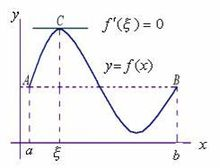
\includegraphics{resources/Rolle's_mean_value_theorem.jpg}

  如果函数$\fint(x)$满足:

  \begin{enumerate}
    \item 在闭区间$[a,b]$上连续;
    \item 在开区间$(a,b)$上可导;
    \item 在区间端点处的函数值相等,即$\fint(a) = \fint(b)$,
  \end{enumerate}

  那么在$(a,b)$内至少有一点$\xi, (a<\xi<b)$,使得$\fint\derivative(\xi) = 0$。这个定理称为罗尔定理
}%罗尔中值定理结尾

\subsubsection{拉格朗日中值定理}{
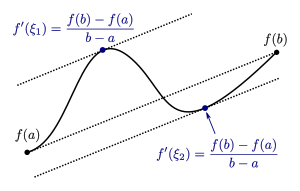
\includegraphics{resources/Lagrange's_mean_value_theorem.png}

令$\fint : [a,b] \to \mathbf{R}$为闭区间$[a,b]$上的一个函数,且在开区间
$(a,b)$内对任意一点$x$,极限$\limNormal{h \to 0}\frac{\fint(x + h) - \fint(x)}{h}$存在,
为一个有限数字或者等于$+\infty$或$-\infty$.如果有限,则极限等于$\fDerivative{x}$。

此定理称为{\bfseries拉格朗日中值定理},也简称中值定理,是罗尔中值定理的更一般的形式,同时也是柯西中值定理的特殊情形

这个定理再可以稍微推广一点。只需假设$\fint : [a,b] \to \mathbf{R}$在$[a,b]$连续,且在开区间$(a,b)$内对任意一点$x$,极限$\limNormal{h \to 0}
  \frac{\defFunction{x + h} - \defFunction{x}}{b - a}$存在,为一个有限数字或者等于$+\infty$或者$-\infty$.如果有限,则极限等于$\fDerivative{x}$。
这版本定理应用的一个例子是函数$x \to x^{\frac{1}{3}}$,实值三次方根函数,其导数在原点趋于无穷。

注意若一个可微函数的值域是复数而不是实数,则上面这定理就未必正确。例如,对实数$x$定义$\defFunction{x} = e^{ix}$。那么

$\defFunction{2\pi} - \defFunction{0} = 0 \neq \fDerivative{c}(2\pi - 0)$

因$|\fDerivative{x}| = 1 \neq 0$时,$c$为开区间$(0,2\pi)$中任意一点。
}%拉格朗日中值定理结尾

\subsubsection{柯西中值定理}{
  柯西中值定理,也叫拓展中值定理,是中值定理的一般形式。它叙述为:如果函数$f$和$g$都在闭区间$[a,b]$上连续,且在开区间$(a,b)$上可微,那么存在某个$c \in (a,b)$,
  使得$(\defFunction{b} - \defFunction{a})g\derivative(c) = (g(b)-g(a))\fDerivative{c}$

  当然,如果$g(a) \neq g(b)$且$g\derivative(c) \neq 0$,则可表示成:$\frac{\fDerivative{c}}{g\derivative(c)} = \frac{\defFunction{b} - \defFunction{a}}{g(b) - g(a)}$

  在几何上,这表示曲线

  $$
    \begin{cases}
      [a,b] \to \mathbf{R}^2 \\
      t \mapsto (f(t), g(t))
    \end{cases}
  $$
  上存在一点其切线平行于由两点$(\defFunction{a}, g(a))$和$(\defFunction{b}, g(b))$所连接的直线。但柯西定理不能表明在任何情况下这种切线都存在,因为可能存在一些c值使$\defFunction{c} = g(c) = 0$, 所以在这些点曲线根本没有切线。
  下面是这种情况的一个例子

  $t \mapsto (t^3, 1-t^2)$

  在区间$[-1,1]$上,曲线由$(-1, 0)$到$(1,0)$,却并无一个水平切线,然而他在$t = 0$出有一个驻点(实际上是一个尖点)。

  柯西中值定理可以用来证明洛必达法则。拉格朗日中值定理是柯西中值定理当$g(t) = t$时的特殊情况。
}%柯西中值定理结尾

}%微分结尾


\subsection{定积分}{

  \subsubsection{区间再现公式}{
    设$\defFunction{x} = \definiteIntegral{a}{b}g(x)dx$,令$x = a + b - t$,当$x = a$时,$t = b$,当$x = b$时,$t = a$,$dx$变成$-dt$。即:

    $\defFunction{x} = \definiteIntegral{a}{b}g(x)dx = -\definiteIntegral{b}{a}g(a+b-t)dt = \definiteIntegral{a}{b}g(a + b - t)dt$

    由于定积分与被积变量无关,所以将上式结果中的t换成x,与原函数相加,得:

    $\defFunction{x} = \frac{1}{2}\definiteIntegral{a}{b}[g(x) + g(a + b - x)]dx$
  }%区间在线公式结尾

}%定积分结尾

}%微积分结尾

\section{高等代数/线性代数}{
\subsection{定义、解释、前言}{
\subsubsection{什么是线性变换}{
  什么是线性变换?线性变换是变换的一种,是操纵抽象的向量空间的手段,通过线性变换可以将空间进行放缩与变形。
  所谓的“线性”意味着这类变换满足以下两个性质:

  \begin{enumerate}
    \item $L(\vec{u}+\vec{v}) = L(\vec{u})+L(\vec{v})$
    \item $L(\mathbf{C}\vec{v}) = \mathbf{C}L(\vec{v})$
  \end{enumerate}

  所谓的线性通常指的就是这回事,而满足线性也通常暗示着某种可能-用矩阵表示对象的可能。
  举个例子,求导就是一种线性运算,它符合以上的两个条件。事实上也并不是只有一次幂的函数可以用线性代数的方法表示。

  正因大部分函数可以表示成矩阵与向量,事实上线性代数的很多概念都在函数中有直接类比,比如:

  \begin{tabular}{c|c}
    \hline
    线性代数中的概念                & 应用于函数时的别名          \\
    \hline
    线性变换(Linear transformation) & 线性算子(Linear operatiors) \\
    点积(Dot products)              & 内积(Inner products)        \\
    特征向量(Eigen vectors)         & 特征函数(Eigen functions)
  \end{tabular}

  可以看出数学中还有很多类似向量的事物。只要所处理对象,具有合理的数乘和加和概念,不管是空间中的箭头、一组数还是函数集合,线性代数中所有关于向量、线性变换和其他的概念都应该适用于它。这些类似向量的事物,它们构成的集合被称为向量空间。这些内容将在“抽象向量空间”章节中讨论
}%线性变换结尾

\subsubsection{关于抽象向量空间}{
为什么要定义这么麻烦的规则?在数学的表达中,我们倾向于得到用普适的概念,{\bfseries而普适的代价就是抽象}。在日常生活中不难发现很多东西都给人一种线性的错觉,事实上那不是错觉,向量也不一定得是箭头或坐标什么的,因此为了规范向量的定义,得到所期望的普适性,抽象出以下规则,这意味着:如果要将一类对象称为向量并且对其运用线性代数的知识,则必须满足以下条件。

(也可以称这堆玩意为向量加法和数乘的规则):
\begin{enumerate}
  \item $\vec{u} + (\vec{v} + \vec{w}) = (\vec{u} + \vec{v}) + \vec{w}$
  \item $\vec{v} + \vec{w} = \vec{w} + \vec{v}$
  \item 存在一个$\vec{0}$使得$\vec{0} + \vec{v} = \vec{v}$,这应该对于所有$\vec{v}$都成立。
  \item 对于所有的$\vec{v}$,都存在$-\vec{v}$,使得$\vec{v} + (-\vec{v}) = \vec{0}$
  \item $a(b\vec{v}) = (ab)\vec{v}$
  \item $1\vec{v} = \vec{v}$
  \item $a(\vec{v} + \vec{w}) = a\vec{v} + a\vec{w}$
  \item $(a + b)\vec{v} = a\vec{v} + b\vec{v}$
\end{enumerate}

在新定义的向量空间中应用线性代数的结论之前,需要验证它的定义是否满足以上要求。

如果要让已经建立好的线代理论和概念适用于一个空间,那么必须满足这8条公理。这8条公理保证新定义的向量,其加法和数乘符合你一直接受的状态。

那么,有了这些明确的规则,就可以在任何{\bfseries符合这些规则}的抽象的向量空间中使用线性代数了。
}%关于抽象向量空间结尾

}%定义、解释、前言结尾

}%高等代数/线性代数结尾

}%数学篇结尾
\end{document}